\chapter{对抗性信息在视觉目标跟踪算法中的应用} \label{chap:attack}
在前面的章节中,我们展示了通过添加语义信息、时空信息和自适应信息,可以有效提高视频跟踪算法的性能。最近有研究显示,孪生跟踪器容易受到对抗性攻击。但是,现有的攻击方法独立地为每个视频制作扰动,这在计算上具有不可忽略的成本。如果在线跟踪阶段无法访问有限的计算资源,则此类攻击方法难以在现实世界中发挥作用。

在本章中,我们展示了与视频无关的扰动的存在,用于对视觉目标跟踪算法执行对抗性攻击,例如强制跟踪器输出指定轨迹。所提出的对抗性扰动信息在不同视频间具有通用性,执行攻击时无需为不同视频重新生成扰动。具体来说,我们通过向模板图像添加通用的不可感知的扰动并将虚假目标(一个通用对抗补丁)根据预定义轨迹粘贴到搜索图像中来攻击跟踪器,使得跟踪器输出虚假目标而非真实目标的位置和大小。本章提出的方法允许仅通过执行加法操作和图像粘贴操作就可以干扰基于孪生网络的视觉目标跟踪算法,而无需进行梯度优化或网络推理。在多个数据集上的实验结果表明,我们的方法可以有效地欺骗孪生跟踪器。

\section{引言}

\begin{figure}[t]
\centering
\subfloat{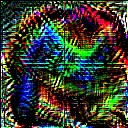
\includegraphics[width=0.3\textwidth]{Img/attack/x.jpg}} \qquad \qquad 
\subfloat{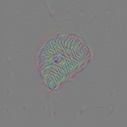
\includegraphics[width=0.3\textwidth]{Img/attack/z.jpg}}
\caption{对抗性信息的可视化结果。左图:为搜索图像生成的对抗补丁。右图:为模板图像生成的对抗扰动。}
\label{fig:attack}
\end{figure}

给定视频初始帧中的任意目标,视觉目标跟踪的任务是在后续帧中对该目标进行识别并定位。
%在线跟踪阶段中从单个初始样本跟踪视觉对象的这种范式最近被广泛地描述为基于孪生网络的单发问题 \cite{SiamFC,SiamRPN,SiamRPN++,SiamFC++},称为
最近提出的孪生网络框架 \cite{SiamFC,SiamRPN,SiamRPN++,SiamFC++} 可有效地处理视觉目标跟踪任务。

近年来,孪生跟踪器的鲁棒性引起了很多关注,并且研究重点已转向设计更有效、计算成本更低的攻击方法 \cite{TTP,FAN,SPARK}。尽管很多攻击方法可以成功地攻击孪生网络跟踪器,但这些攻击方法仍不适合以有限的计算资源来攻击基于低功耗计算平台构建的在线跟踪系统,原因是这些攻击方法需要基于迭代优化或对抗生成网络推理来独立地为每个视频制作扰动。因此,在计算密集型的跟踪系统中可能无法确保计算资源充足可用。

在文献 \cite{UAP} 中,作者提出的通用对抗性扰动(universal adversarial perturbation,UAP)能够以与图像无关的方式欺骗同一数据分布中的大多数图像。UAP 具有通用性,可以用于快速扰动数据,而无需进行额外计算。因此,攻击在计算资源有限的平台上部署的实时应用程序时,UAP 具有重要作用。然而,很少有工作研究如何使用 UAP 攻击孪生跟踪器,因为很难将现有的 UAP 直接应用于攻击孪生跟踪器。主要原因在于:
\begin{itemize}
\item 大多数 UAP 是为传统神经网络架构设计的,该架构接受一幅图像作为输入,而孪生网络同时接受模板图像和搜索图像作为输入。
\item 现有的 UAP 方法往往用于干扰模型的二进制输出,而我们需要使用通用扰动使得孪生跟踪器输出指定的轨迹。
\end{itemize}

在本章中,我们提出为主流的孪生跟踪器 SiamFC++ \cite{SiamFC++} 生成视频无关的通用对抗性扰动信息(图 \ref{fig:attack})。具体而言,我们旨在通过向模板图像添加通用的不可感知的扰动并将虚假目标(即小的通用对抗补丁)根据预定义轨迹粘贴到搜索图像中来攻击跟踪器(图 \ref{fig:1}),使得跟踪器输出虚假目标而非真实目标的位置和大小。利用本章提出的视频无关的通用扰动攻击一段新视频时,仅需执行加法操作和图像粘贴操作即可,而无需执行梯度优化或网络推理,因此几乎不会增加计算成本。在 OTB2015 \cite{OTB2015},GOT-10k \cite{GOT-10k} 和 LaSOT \cite{LaSOT} 基准测试数据库上的实验结果证明了我们方法的有效性。
%\nopagebreak[4]
\section{相关工作}

\begin{figure}[t]
\centering
%\subfigure{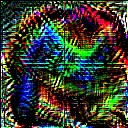
\includegraphics[width=0.2\textwidth]{Img/attack/x.jpg}} \qquad
%\subfigure{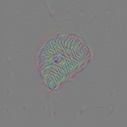
\includegraphics[width=0.2\textwidth]{Img/attack/z.jpg}}
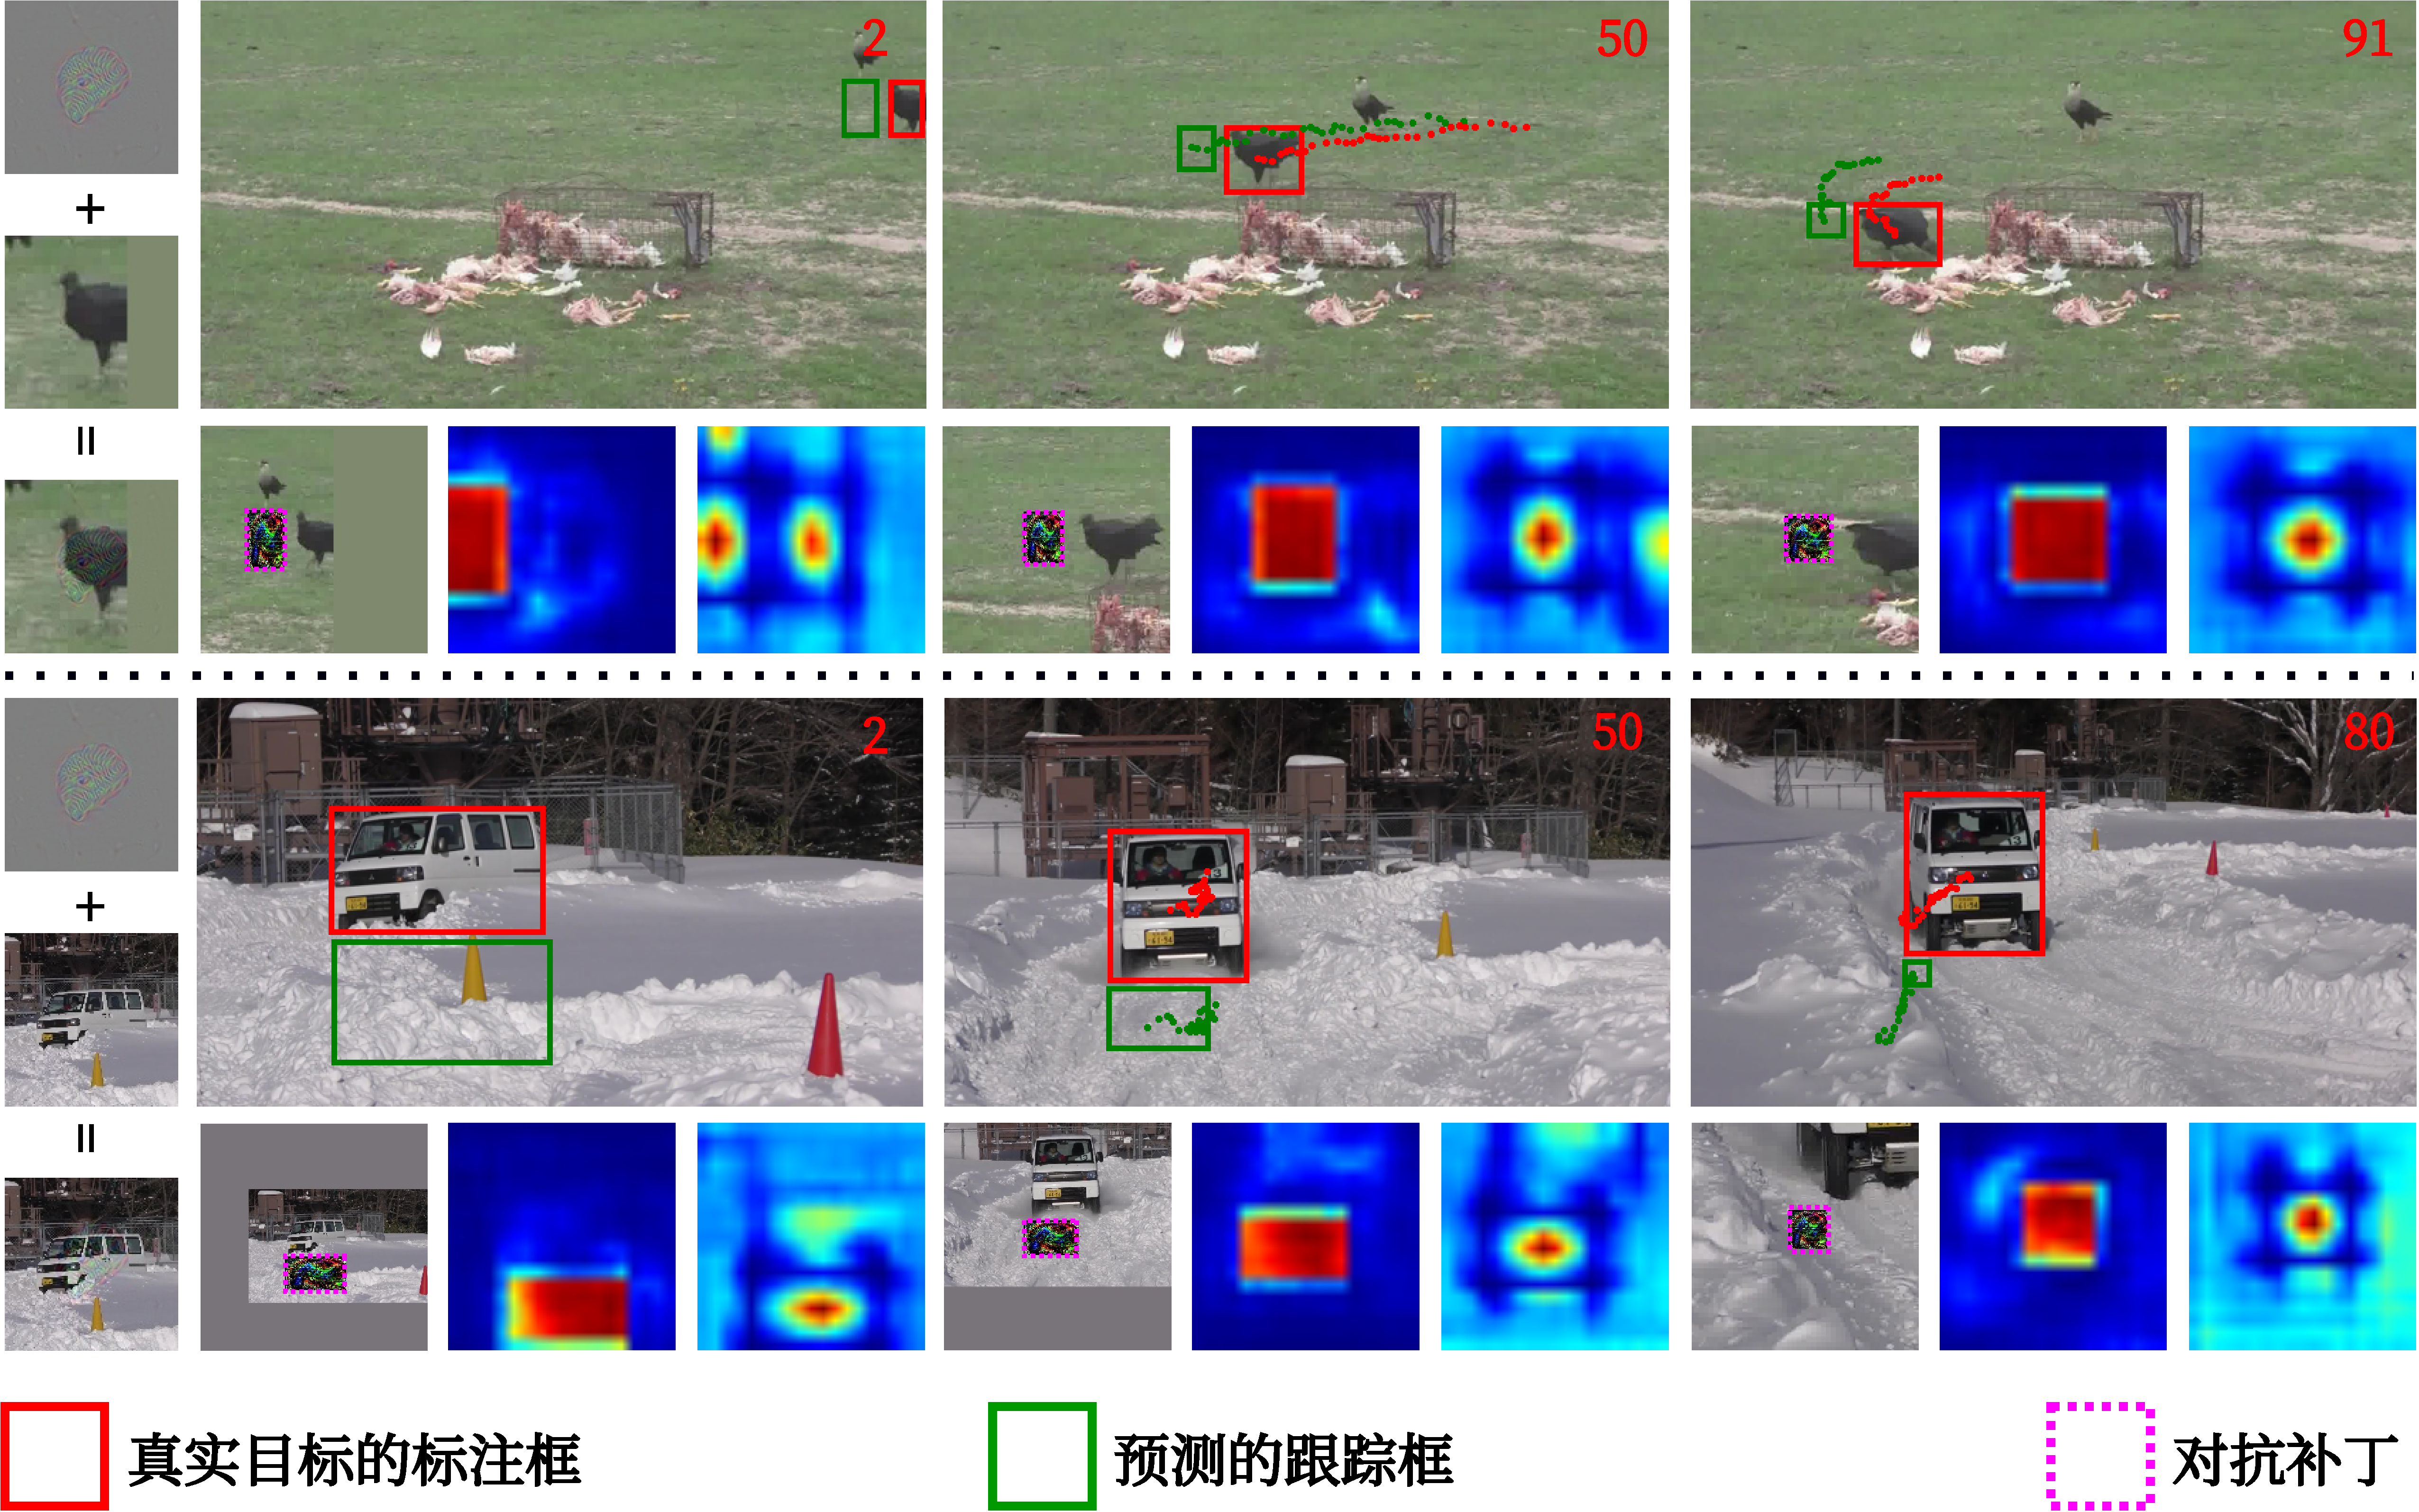
\includegraphics[width=1.0\textwidth]{Img/attack/1_v8.pdf}
\caption{在 GOT-10k 视频目标数据库中的一些视频序列上展示本章算法对 SiamFC++ 的攻击效果。我们的方法会产生视频无关的通用扰动,用于迫使 SiamFC++ 遵循复杂的轨迹,而几乎不会增加任何计算量。对抗性信息通过离线训练获得。跟踪器错误地认为虚假目标区域包含要跟踪的目标(请参见左侧的热图)。此外,对抗性信息还同时误导了 SiamFC++ 中的质量评估分支(请参见右侧的热图)。注意,虚假目标的大小逐渐减小。} 
%Being universal, the generated perturbations can be conveniently exploited to perturb videos on-the-fly without extra computations. 
%Red represents the ground-truth bounding box, and green represents the predicted bounding box by the tracker.
%The purple dashed box marks the universal adversarial patch. The left heatmap represents the probability of each spatial position to contain the \textit{fake target}, and the right heatmap represents the target state estimation quality.}
\label{fig:1}
\end{figure}

\subsection{孪生网络跟踪器}

基于模板匹配思想的跟踪算法主要包括基于相关滤波器的视觉目标跟踪算法和基于孪生网络的视觉目标跟踪算法。两者都旨在估计从初始视频帧裁剪的模板在后续帧中的位置。孪生跟踪器将视觉跟踪形式化为以卷积方式学习目标模板和搜索区域中候选目标之间的相似性。搜索图像区域中具有最高视觉相似度的位置被确定为目标位置。

最近,一些孪生跟踪器~\cite{SiamRPN,SiamRPN++,SiamFC++} 已证明,孪生网络架构可为视觉目标跟踪带来显著的性能改进。
具体而言,SiamRPN \cite{SiamRPN} 由一个用于特征提取的孪生子网络和一个分别包含分类和回归分支的区域生成子网络组成。SiamRPN++ \cite{SiamRPN++} 基于对分类任务和状态估计任务的分解,通过一种简单而有效的空间感知采样策略突破了严格的平移不变性的限制,并成功地训练了 ResNet 驱动的孪生跟踪器,从而显著提高了性能。除了这些基于锚框的方法以外,Xu 等人 \cite{SiamFC++} 进一步设计了无锚跟踪器 SiamFC++。在本章的实验中,我们将重点放在无锚的 SiamFC++ 跟踪器上,同时分析了对抗性信息在基于锚框的跟踪器上的可迁移性。

\subsection{对抗攻击}

在文献 \cite{intriguing} 中首次研究了图像分类的对抗性攻击,目的是指出现代深度卷积神经网络对不可感知的扰动的脆弱性。
%Recent studies also emerge to investigate the adversarial attacks to other diverse types of tasks such as natural language processing \cite{generating} and object detection \cite{wei2019transferable}.
最近很多研究将对抗性信息的应用扩展到其他领域,如自然语言处理 \cite{generating} 和图像目标检测 \cite{wei2019transferable}。
可以按照不同的维度将对抗性信息进行分类。

\textbf{不可感知的扰动与对抗补丁} 不可感知的扰动通常会使每个像素发生少量变化,并且可以使用多种优化策略进行求解,例如 BFGS \cite{intriguing} 和 PGD \cite{PGD}。
对抗补丁可以放置在输入图像中的任何位置,以引起网络行为异常,因此常用于通用攻击 \cite{patch}。
在本章中,我们同时利用不可感知的扰动和对抗补丁来攻击目标跟踪器,两种不同形式的扰动以端到端的方式共同训练。
此外,本章提出的对抗性扰动信息在网络域而不是图像域中工作。在网络域设置中,扰动可以取任何值,并且不受图像像素取值范围的约束 \cite{karmon2018lavan}。

\textbf{非针对性攻击与针对性攻击} 在非针对性攻击的情况下,攻击者的目标是使网络预测任何不正确的标签,而不关注标签的具体取值,例如在视觉目标跟踪中使估计的目标位置远离真实目标位置。
针对性攻击任务的目的是将网络的预测更改为某个特定的标签。在视觉目标跟踪任务中,针对性攻击旨在误导跟踪器按照预定的轨迹输出目标位置。

\subsection{视觉目标跟踪中的对抗攻击}

最近,多项研究工作对视觉目标跟踪任务的对抗攻击进行了探索。例如,PAT \cite{PAT} 通过白盒攻击生成物理对抗纹理,以引导跟踪器在被跟踪目标移到纹理前面时锁定跟踪框。然而,PAT 仅通过攻击跟踪器 GOTURN \cite{GOTURN} 来验证其方法的有效性,该跟踪器与主流的目标跟踪算法相比在性能上有较大差距。在本章中,我们旨在攻击最先进的孪生跟踪器。
RTAA \cite{RTAA} 利用时间信息为视频的每帧图像生成微小扰动。然而,RTAA 仅对跟踪器执行非针对性攻击。相比之下,本章中的针对性攻击更具挑战性,因为我们的目标是在测试时令跟踪器遵循任意的复杂轨迹。
SPARK \cite{SPARK} 通过使用过去帧中的信息计算增量扰动以对孪生跟踪器进行针对性攻击。然而,SPARK 需要通过繁琐的迭代计算为每个搜索图像生成独特的对抗样本,这对于实时在线跟踪算法而言非常耗时。在文献 \cite{TTP} 中,Nakka 等人提出仅使用模板图像生成一个时间可传递的扰动,然后将其添加到每个搜索图像中,以进行实时攻击。然而,该方法针对每个视频都需要运行对抗生成网络以计算特定于视频的扰动。当计算资源有限或无法访问时,便不适用于攻击现实世界中的在线跟踪系统。因此在本章中,我们提出了与视频无关的通用扰动,该扰动允许仅通过加法操作和图像粘贴操作即可对任意视频进行扰动,因此几乎不会增加计算成本。

\begin{figure}[t]
\centering
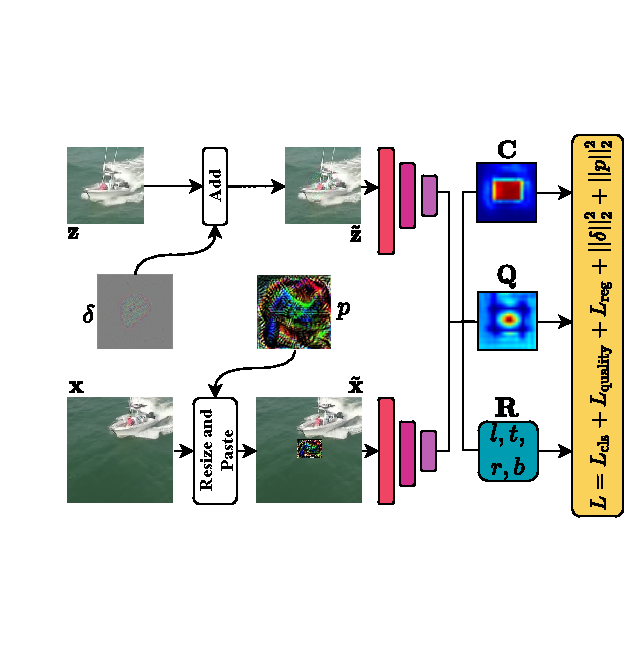
\includegraphics[width=0.75\textwidth]{Img/attack/network_v5.pdf}
\caption{所提出方法的训练流程。我们旨在为模板图像 $\textbf z$ 训练难以感知的扰动 $\delta$ ,为搜索图像 $\textbf x$ 训练对抗补丁 $p$ 。在将 $\delta$ 添加到 $\textbf z$ 并将虚假目标 $p$ 粘贴到 $\textbf x$ 之后,跟踪器将输出虚假目标而非真实目标的位置和大小。}
\label{fig:net}
\end{figure}

\section{对抗性信息在孪生跟踪器中的应用}
在本节中,我们提出针对孪生跟踪器的视频无关的对抗攻击框架,旨在通过向模板图像添加不可感知的扰动并将虚假目标(即对抗补丁)根据预定义轨迹粘贴到搜索图像中来攻击跟踪器,以便跟踪器输出虚假目标而非真实目标的位置和大小。接下来,我们将形式化孪生网络 \cite{SiamFC++} 的针对性攻击问题,然后详细介绍我们的扰动策略。

\subsection{问题定义}
令 $V=\{I_i\}_1^T$ 表示长度为 $T$ 的视频序列。
$B^{gt}=\{b^{gt}_i\}_1^T$ 用于表示目标在每一帧中的真实位置。
视觉目标跟踪旨在给定目标初始状态的情况下,在随后的帧中预测此目标的位置 $B^{pred}=\{b^{pred}_i\}_1^T$。
在 SiamFC++ 中,跟踪器首先将参考帧 $I_1$ 根据对应的注释边界框 $b_1^{gt}$ 转换为模板图像 $\textbf z$,然后将搜索帧 $I_i$ 转换为以上一帧中估计的位置为中心的搜索图像 $\textbf x_i$。
在每个时刻,模板图像 $\textbf z$ 和搜索图像 $\textbf x_i$ 首先分别通过共享的主干网络提取特征,然后使用逐通道互相关操作对其进行融合:
\begin{equation}
f_{j}(\textbf z, \textbf x_i)=\psi_{j}(\phi(\textbf z)) \star \psi_{j}(\phi(\textbf x_i)), j \in\{\mathrm{cls}, \mathrm{reg}\}.
\end{equation}
其中,$\star$ 表示逐通道互相关操作,$\phi(\cdot)$ 表示孪生网络的特征提取器,$\psi_j(\cdot)$ 表示特定于分类或回归任务的层,$j$ 表示特定任务类型($\mathrm{cls}$ 表示分类任务,$\mathrm{reg}$ 表示回归任务)。$\psi_{\mathrm{cls}}$ 和 $\psi_{\mathrm{reg}}$ 均设计为两个卷积层,用于将通用特征调整到特定于分类/回归任务的特征空间。$\psi_{\mathrm{cls}}$ 和 $\psi_{\mathrm{reg}}$ 所提取的特征具有相同尺寸。
融合后的特征随后送入子网络中,以无锚的方式预测分类图 $\textbf{C}$,边界框回归图 $\textbf{R}$ 和质量评估图 $\textbf{Q}$。简而言之,$\textbf C$ 编码每个空间位置包含目标的概率,$\textbf R$ 回归目标的边界框,而 $\textbf Q$ 预测目标状态质量评估得分。最后,根据 $\textbf{C}$,$\textbf{R}$ 和 $\textbf{Q}$ 生成目标边界框。

我们的任务是为模板图像 $\textbf z$ 训练不可感知的扰动 $\delta$,为搜索图像 $\textbf x_i$ 训练对抗补丁 $p$。在将 $\delta$ 添加到 $\textbf z$ 并将虚假目标 $p$ 粘贴到 $\textbf x_i$ 之后,跟踪器将输出对抗补丁而非真实目标的位置和大小(请参见图 \ref{fig:net})。
$\delta$ 和 $p$ 是通用的(即与视频无关),这意味着扰动一段新的视频仅需将扰动添加/粘贴到模板/搜索图像上,而无需进行梯度优化或网络推断。

\subsection{产生视频无关的对抗扰动}
在本节中,我们展示如何为孪生跟踪器训练与视频无关的扰动 $(\delta, p)$。在训练的第 $k$ 次迭代中,从训练数据集 $\mathcal V$ 中随机选择一段视频 $V=\{I_i\}_1^T$。假设第 $k$ 次迭代的模板扰动是 $\delta_k \in \mathbb{R}^{127\times 127 \times 3}$,对抗补丁是 $p_k \in \mathbb{R}^{128\times 128\times 3}$。我们首先从 $V$ 中随机选择两帧 $I_t, I_s$。
干净的模板图像 $\textbf z\in \mathbb{R}^{127\times 127 \times 3}$ 是根据 $I_t$ 和 $b^{gt}_t$ 生成的,扰动后的模板图像为:
\begin{equation}
\tilde {\textbf z} = \textbf z + \delta_k.
\end{equation}
类似地,干净的搜索图像 $\textbf x \in \mathbb{R}^{303\times 303 \times 3}$ 是根据 $I_s$ 和 $b^{gt}_s$ 生成的。
如前所述,对抗补丁被视为虚假目标并粘贴到搜索图像中。我们使虚假目标的中心位置靠近真实目标的中心位置(具有最大 64 个像素的随机平移)。
虚假目标的宽度/高度介于 32 像素和 128 像素之间。
扰动后的搜索图像生成如下:
\begin{equation}
\tilde{\textbf x} = A(\textbf x, p_k, (l^x, l^y), (w, h)),
\end{equation}
其中 $(l^x, l^y)$ 和 $(w, h)$ 分别表示虚假目标相对于搜索图像的位置和大小。$A$ 是补丁粘贴操作 \cite{patch},该操作首先将补丁 $p_k \in \mathbb{R}^{128\times 128\times 3}$ 的大小调整为 $\hat{p}_k \in \mathbb{R}^{w\times h\times 3}$,然后将调整过大小的补丁 $\hat{p}_k$ 粘贴到搜索图像 $\textbf x$ 的 $(l^x,l^y)$ 位置。

随后,我们将 $\tilde {\textbf x}$ 和 $\tilde{\textbf z}$ 输入 SiamFC++ 跟踪器,并得到融合特征 $f_{\mathrm{cls}}(\tilde{\textbf z}, \tilde {\textbf x})$ 和 $f_{\mathrm{reg}}(\tilde{\textbf z}, \tilde {\textbf x})$。

遵循 SiamFC++ \cite{SiamFC++} 中将分类任务和回归任务解耦的设计准则,在嵌入空间执行逐通道互相关后,融合特征分别被送入分类分支和回归分支。分类分支将 $f_{\mathrm{cls}}$ 作为输入,对于互相关得到的特征图中的每一个像素,判断该像素对应图像块为正样本或负样本。类似地,回归分支将 $f_{\mathrm{reg}}$ 作为输入,并输出额外的回归偏移量以对预测的边界框位置进行优化。

对于分类分支,特征图 $f_{\mathrm{cls}}$ 上任意空间位置 $(x,y)$ 对应于输入图像上的位置为 $\left(\left\lfloor\frac{s}{2}\right\rfloor+x s,\left\lfloor\frac{s}{2}\right\rfloor+y s\right)$。如果该位置落入虚假目标的标注框内,则认为 $(x,y)$ 是正样本,反之则认为是负样本。$s=8$ 表示特征提取网络的总步长。

在回归分支中,最后一个卷积层预测位置 $\left(\left\lfloor\frac{s}{2}\right\rfloor+x s,\left\lfloor\frac{s}{2}\right\rfloor+y s\right)$ 到虚假目标标注框的四个边的距离,表示为四维向量 $\boldsymbol{t}^{*}=\left(l^{*}, t^{*}, r^{*}, b^{*}\right)$。因此,位置 $(x,y)$ 的回归标签可表示为:

\begin{equation}
\begin{array}{ll}
l^{*}=\left(\left\lfloor\frac{s}{2}\right\rfloor+x s\right)-x_{0}, \quad t^{*}=\left(\left\lfloor\frac{s}{2}\right\rfloor+y s\right)-y_{0} \\
r^{*}=x_{1}-\left(\left\lfloor\frac{s}{2}\right\rfloor+x s\right), \quad b^{*}=y_{1}-\left(\left\lfloor\frac{s}{2}\right\rfloor+y s\right)
\end{array}
\end{equation}
其中,$(x_0, y_0)$ 和 $(x_1, y_1)$ 分别表示虚假目标标注框 $B^*$ 的左上角和右下角坐标。

分类和回归分支的特征图中的每个位置 $(x,y)$,都对应于输入图像中以位置 $\left(\left\lfloor\frac{s}{2}\right\rfloor+x s,\left\lfloor\frac{s}{2}\right\rfloor+y s\right)$ 为中心的图像块。SiamFC++ \cite{SiamFC++} 直接对该位置对应的图像块进行分类,并在该位置上回归目标边框位置。换句话说,SiamFC++ 直接将位置作为训练样本。然而,在基于锚框的跟踪器中,将输入图像上的位置视为多个锚框的中心,为同一位置输出多个分类得分,并相对锚框进行边框回归,从而导致目标与锚框的匹配产生歧义。因此在 SiamFC++ 中,以逐像素的方式进行预测,从而仅为特征图上的每个像素进行一次预测。每个分类得分直接表明该位置对应的图像区域的目标置信度。由于 SiamFC++ 不利用预定义的锚框,而是根据位置进行分类和回归,因此没有关于目标分布的任何先验知识(如尺度、长宽比等),提高了算法的泛化性。

\begin{algorithm}[tb]
\caption{训练过程}
\label{alg:algorithm}
\textbf{输入}: 训练数据集 $\mathcal{V}$ 和最大迭代次数 $N$。\\
\textbf{输出}: 不可感知的扰动 $\delta$ 和对抗补丁 $p$。
\begin{algorithmic}[1] %[1] enables line numbers
\State 令 $k = 0$。
\While{$k < N$}
\State 随机选择一段视频 $V\in \mathcal{V}$。对应的真实标注为 $B^{gt}=\{b^{gt}_i\}^T_1$。
\State 从 $V$ 中随机选择一对帧 $I_t, I_s$。
\State 根据 $I_t$ 和 $b^{gt}_t$ 生成模板图像 $\textbf{z}$。
\State $\tilde{\textbf{z}} = \textbf{z} + \delta_k$。
\State 根据 $I_s$ 和 $b^{gt}_s$ 生成搜索图像 $\textbf{x}$。
\State 计算虚假目标相对于搜索图像的位置 $\{l^x, l^y, w, h\}$。
\State $\tilde{\textbf x} = A(\textbf x, p_k, (l^x, l^y), (w, h))$。
\State 将 $(\tilde{\textbf{z}}, \tilde{\textbf x})$ 送入孪生跟踪器并得到输出 $\textbf{C, R, Q}$。
\State 使用 $\{l^x, l^y, w, h\}$ 生成虚假标签 $\textbf{C}^*,\textbf{R}^*,\textbf{Q}^*$。
\State 使用公式 \ref{eq:loss} 计算损失 $L(\textbf{C, R, Q}, \textbf{C}^*, \textbf{R}^*, \textbf{Q}^*)$。
\State $\delta_{k+1} = \delta_{k} - \epsilon_1 \cdot \text{sign}(\nabla_{\delta_k}L)$。
\State $p_{k+1} = p_{k} - \epsilon_2 \cdot \text{sign}(\nabla_{p_k}L)$。
\State $k = k + 1$。
\EndWhile
\State \textbf{返回} $\delta_N, p_N.$
\end{algorithmic}
\label{attack_alg}
\end{algorithm}

如果仅使用分类得分选择最终的目标框,可能会导致定位精度的降低。因为 Jiang 等人 \cite{IoU-Net} 表明分类置信度与定位精度没有很好的相关性。根据 Luo 等人 \cite{ERF} 的分析,位于子窗口中心附近的像素在相应的输出特征上具有更高的重要性。因此,SiamFC++ 假设目标中心附近的特征像素将比其他像素具有更高的重要性。遵循 SiamFC++ 的设计,我们利用一个 $1 \times 1$ 卷积层进行质量评估,即学习预测边框与虚假目标标注框的交并比(intersection over union,IoU)得分:
\begin{equation}
\mathrm{IoU}^{*}=\frac{\text { Intersection }\left(b, b^{*}\right)}{\operatorname{Union}\left(b, b^{*}\right)}
\end{equation}

测试时,用于最终目标框选择的得分通过质量评估得分与分类得分相乘得出。因此,远离目标中心的边界框将具有较低的权重。

\begin{figure*}[t]
\centering
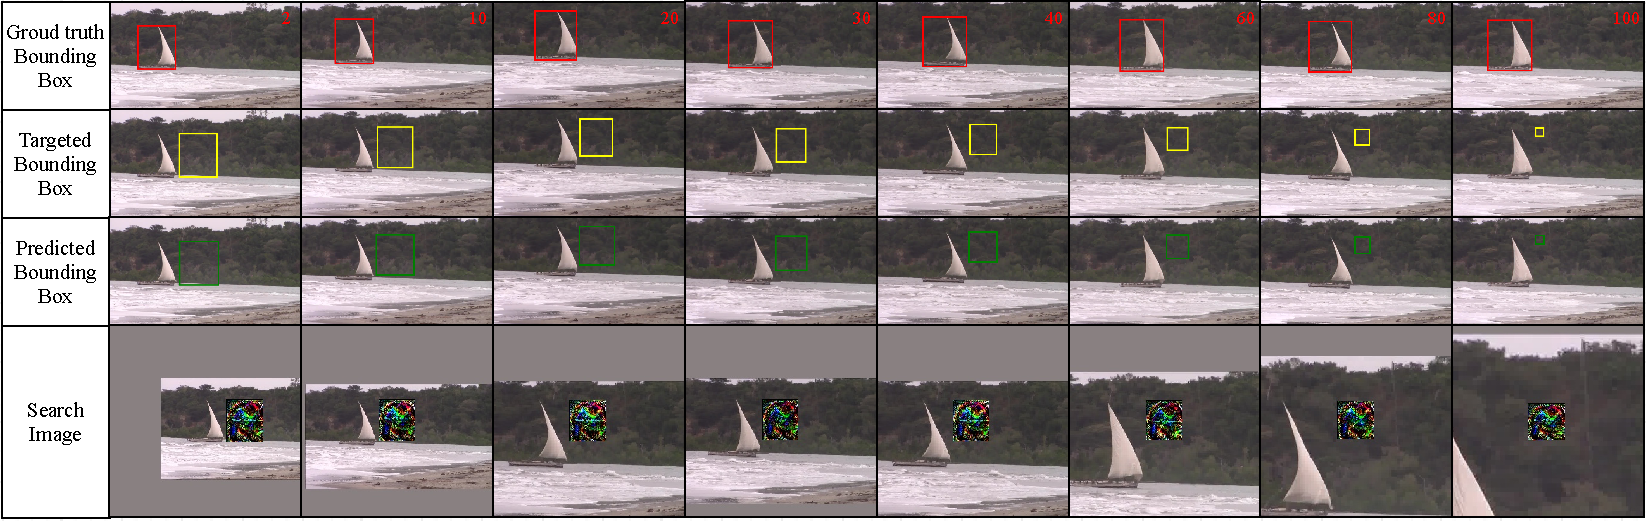
\includegraphics[width=1.0\textwidth]{Img/attack/vis_v4.pdf}
\caption{对抗攻击效果展示。所提出的对抗性信息可使孪生跟踪器沿预定义的虚假轨迹(黄色边框)输出跟踪结果。}
\label{fig:attack_vis}
\end{figure*}

\textbf{训练目标} 损失函数的计算如下:
\begin{equation}
\begin{array}{l}
\begin{aligned}
L&=\frac{\alpha}{N_{\mathrm{pos}}} \sum_{x, y} L_{\mathrm{cls}}\left(\textbf{C}_{x, y}, \textbf{C}_{x, y}^{*}\right) \\
&+\frac{\beta}{N_{\mathrm{pos}}} \sum_{x, y} \textbf{1}_{\left\{\textbf{C}_{x, y}^{*}>0\right\}} L_{\mathrm{quality}}\left(\textbf{Q}_{x, y}, \textbf{Q}_{x, y}^{*}\right) \\
&+\frac{\gamma}{N_{\mathrm{pos}}} \sum_{x, y} \textbf{1}_{\left\{\textbf{C}_{x, y}^{*}>0\right\}} L_{\mathrm{reg}}\left(\textbf{R}_{x, y}, \textbf{R}_{x, y}^{*}\right) \\
&+\eta \cdot ||\delta_k||_2^2 +  \sigma \cdot ||p_k||^2_2,
\end{aligned}
\end{array}
\label{eq:loss}
\end{equation}
\textcolor{black} %(SiamFC++)
{其中 $\textbf{C}_{x, y}, \textbf{R}_{x, y}, \textbf{Q}_{x, y}$ 分别表示 $\textbf{C}, \textbf{R}, \textbf{Q}$ 在位置 $(x, y)$ 的值。$\textbf{C}^*, \textbf{R}^*, \textbf{Q}^*$ 是根据虚假目标的位置和大小生成的虚假标签。$\textbf 1$ 是指示函数,如果条件成立,则取 1,否则将取 0。$N_{\mathrm{pos}}$ 表示训练阶段正样本的数量,$L_{\mathrm{cls}}$ 表示分类的焦点损失 \cite{focal},$L_{\mathrm{quality}}$ 表示质量评估的二元交叉熵(BCE)损失,$L_{\mathrm{reg}}$ 表示边界框回归的 IoU 损失 \cite{iou-loss}。根据文献 SiamFC++,如果将 $(x, y)$ 视为正样本,则将 1 分配给 $\textbf{C}_{x, y}^{*}$,如果视为负样本,则分配 0。}

\textbf{优化} 在每个训练步骤中,扰动更新如下:
\begin{gather}
\delta_{k+1} = \delta_{k} - \epsilon_1 \cdot \text{sign}(\nabla_{\delta_k}L)\\
p_{k+1} = p_{k} - \epsilon_2 \cdot \text{sign}(\nabla_{p_k}L),
\end{gather}
其中 $\epsilon_1$ 用于确保添加到模板图像的扰动难以感知,而 $\epsilon_2$ 用于确保训练稳定性。
在训练期间,我们仅优化扰动 $(\delta, p)$ 的值,而孪生网络的参数保持不变。
我们在算法 \ref{attack_alg} 中概述了该训练过程。

\begin{table}[t]
\centering
\caption{本章提出的算法在数据集 OTB2015 \cite{OTB2015}、GOT-Val \cite{GOT-10k}、LaSOT \cite{LaSOT} 上的攻击效果。}
\begin{tabular}{c c c c c}
\toprule
\multirow{2}{*}[-2pt]{数据集} & \multirow{2}{*}[-2pt]{评价指标} & 原始图像 & \multicolumn{2}{c}{对抗图像}  \\
\cmidrule(lr){3-3} \cmidrule(lr){4-5}
                          &                         & 真实轨迹 & 真实轨迹 & 虚假轨迹     \\ 
\midrule
\multirow{2}{*}{OTB2015 \cite{OTB2015}} 
& AO   & 0.642 & 0.035 & 0.842\\
& Precision & 0.861 & 0.048 & 0.928\\
\midrule
\multirow{2}{*}{GOT-Val \cite{GOT-10k}} 
& SR & 0.897 & 0.023 & 0.890\\
& AO 				   & 0.760 & 0.035 & 0.818 \\
\midrule
\multirow{3}{*}{LaSOT \cite{LaSOT}} 
& Precision       & 0.514 & 0.013 & 0.820\\
& Norm. Prec. & 0.551 & 0.015 & 0.788\\
& AO & 0.525 & 0.022 & 0.767\\
%& Succ. rate  & 0.626 & 0.016 & 0.834\\
\midrule
\multicolumn{2}{c}{FPS} & 58 & 58 & 58\\
\bottomrule
\end{tabular}
%}
\label{tab:attack_benchmark results}
\end{table}

\subsection{在推理时攻击跟踪器}

一旦对扰动 $(\delta, p)$ 进行了训练,便可用于对基于孪生网络的视觉目标跟踪算法的攻击。$\delta$ 和 $p$ 都是通用的(即与视频无关),这意味着对一段新视频进行扰动仅需将扰动添加/粘贴到模板/搜索图像上,而无需进行梯度优化或网络推断。
假设 $B^{fake}=\{b^{fake}_i\}_1^{T}$ 是希望跟踪器输出的指定轨迹。
在跟踪视频 $V=\{I_i\}_1^T$ 的第 $i$ 帧期间,我们需要将相对于原始帧 $I_i$ 的边界框 $b^{fake}_i$ 变换为相对于搜索图像 $\textbf x_i$ 的边界框 $\hat b_i=\{l^x_i, l^y_i, w_i, h_i\}$ 中,然后根据 $\hat b_i$ 将 $p$ 粘贴到 $\textbf x_i$ :
\begin{equation}
\tilde{\textbf x}_i = A(\textbf x_i, p, (l^x_i, l^y_i), (w_i, h_i)).
\end{equation}
跟踪器将 $\tilde{\textbf z}=\textbf z+\delta$ 和 $\tilde{\textbf x}_i$ 作为输入,随后的跟踪过程与 SiamFC++ 相同。

\section{实验评估与分析}
\subsection{实验设置}

\textbf{测试数据集} 我们在几种跟踪基准,即 OTB2015 \cite{OTB2015}、GOT-10k \cite{GOT-10k} 和 LaSOT \cite{LaSOT} 上评估针对跟踪器的对抗攻击效果。具体而言,OTB2015 是典型的跟踪基准数据库,已被广泛用于跟踪性能评估中。GOT-10k 具有更多的目标类别,LaSOT 具有更长的视频序列,平均持续时间为 84 秒。它们都遵循单次通过评估(OPE)协议,具有相似的评价指标,主要基于跟踪器在测试视频上的跟踪效果衡量其成功率与精确度。

\begin{table}[t]
\centering
\caption{在 GOT-Val 数据集上分析不同损失函数对跟踪性能的影响。}
\begin{tabular}{ccccccc} 
\toprule
\multirow{2}{*}[-2pt]{分类损失}     & \multirow{2}{*}[-2pt]{质量评估损失} & \multirow{2}{*}[-2pt]{回归损失} & \multicolumn{2}{c}{虚假轨迹}          & \multicolumn{2}{c}{真实轨迹}           \\ 
\cmidrule(lr){4-5} \cmidrule(lr){6-7}
                       &                    &                    & AO                    & SR                    & AO                    & SR                     \\ 
\midrule
\checkmark   &    &    & 0.718  & 0.824    & 0.086 & 0.083   \\
   & \checkmark   &    & 0.044  & 0.044    & 0.703 & 0.842   \\
   &    & \checkmark   & 0.664  & 0.726    & 0.165 & 0.184   \\
\checkmark   & \checkmark   & \checkmark   & 0.818  & 0.890    & 0.035 & 0.023   \\ \bottomrule
\end{tabular}
%}
\label{tab:attack_loss}
\end{table}

\textbf{生成虚假轨迹} 我们需要为每个视频预先定义特定的轨迹 $B^{fake}=\{b^{fake}_i\}_1^{T}$,以实现在线跟踪中的针对性攻击,我们称之为虚假轨迹。我们将使用真实边界框表示的真实轨迹定义为 $B^{gt}=\{b^{gt}_i\}_1^T$。
我们可以为每个视频手动标记任意虚假轨迹 $B^{fake}$ ,然而这将非常耗时。因此,我们基于 $B^{gt}$ 生成 $B^{fake}$。具体来说,虚假轨迹沿真实轨迹运动,且 $b^{fake}_i$ 和 $b^{gt}_i$ 的边界相距 16 像素。
%The size of $b^{fake}_0$ is the same as $B^{gt}_0$ and the size of $b^{fake}_i$
虚假轨迹的边框尺寸由 $b^{gt}_1$ 的尺寸逐渐变为 $64\times 64$。由于 GOT-10k 测试集的边界框注释信息未公开,因此我们仅使用 GOT-10k 的验证集进行评估,并将其表示为 GOT-Val。

\textbf{图像质量评估} 我们使用结构相似性(SSIM)\cite{SSIM} 来评估生成的不可感知的模板扰动 $\delta$ 的质量。当 SSIM 接近 1 说明生成的扰动难以感知(请参见表 \ref{tab:attack_iter})。

\textbf{实现细节} 本章采用的基线跟踪器为 SiamFC++ \cite{SiamFC++},其主干孪生网络采用 GoogLeNet \cite{GoogLeNet}。
我们使用 Pytorch 进行算法实现,并使用三个 GTX 1080Ti GPU 训练扰动。
我们采用 COCO \cite{COCO}、ILSVRC-VID \cite{VID} 数据集,以及 GOT-10k \cite{GOT-10k} 与 LaSOT \cite{LaSOT} 的训练集作为训练数据。
以 96 个图像的批次大小(每个 GPU 32 个图像)迭代进行 32768 次训练。
用于生成模板扰动的学习率 $\epsilon_1$ 设置为 0.1,用于生成对抗补丁的学习率为 $\epsilon_2 = 0.5$。
我们按照 SiamFC++ 的方法生成训练样本。
在训练和在线跟踪阶段,SiamFC++ 跟踪网络模型
%\footnote{由 SiamFC++ 的作者使用 GOT-10k 训练集进行训练,可以从 \url{https://drive.google.com/file/d/1BevcIEZr_kgyFjhxayOFw08DFl2u5Zi7/view} 中下载。}
是固定的,并用于整个评估流程。模板图片的空间分辨率设置为 $127\times 127$,搜索图片的空间分辨率设置为 $303\times 303$。
在公式 \ref{eq:loss} 中,设置 $\alpha=1, \beta=1, \gamma=1, \eta=0.005$ 和 $\sigma=10^{-5}$。

\begin{table}[t!]
\centering
\caption{在 GOT-Val 数据集上验证训练迭代次数对攻击效果的影响。}
\begin{tabular}{@{}llllll@{}}
\toprule
\multirow{2}{*}{迭代次数} & \multicolumn{2}{c}{虚假轨迹} & \multicolumn{2}{c}{真实轨迹} & \multirow{2}{*}{SSIM}\\ \cmidrule(lr){2-3} \cmidrule(lr){4-5}
 & \multicolumn{1}{c}{AO} & \multicolumn{1}{c}{SR} & \multicolumn{1}{c}{AO} & \multicolumn{1}{c}{SR} &  \\ \midrule
1 & 0.002 & 0 & 0.757 & 0.894 & 1   \\
2 & 0.002 & 0 & 0.756 & 0.891 & 1   \\
4 & 0.002 & 0 & 0.757 & 0.893 & 1   \\
8 & 0.002 & 0 & 0.757 & 0.891 & 1   \\
16 & 0.002 & 0 & 0.758 & 0.893 & 0.99 \\
32 & 0.003 & 0.001 & 0.759 & 0.896 & 0.99 \\
64 & 0.007 & 0.005 & 0.753 & 0.888 & 0.97 \\
128 & 0.042 & 0.044 & 0.72 & 0.852 & 0.93 \\
256 & 0.299 & 0.335 & 0.474 & 0.559 & 0.86 \\
512 & 0.668 & 0.749 & 0.15 & 0.164 & 0.86 \\
1024 & 0.746 & 0.822 & 0.095 & 0.098 & 0.87 \\
2048 & 0.781 & 0.855 & 0.071 & 0.066 & 0.88 \\
4096 & 0.798 & 0.872 & 0.041 & 0.031 & 0.88 \\
8192 & 0.82 & 0.895 & 0.032 & 0.021 & 0.88 \\
16384 & 0.821 & 0.897 & 0.032 & 0.022 & 0.88 \\
32768 & 0.818 & 0.89 & 0.035 & 0.023 & 0.88 \\ \bottomrule
\end{tabular}
\label{tab:attack_iter}
\end{table}

\subsection{针对孪生跟踪器的攻击效果评估}
\begin{figure}[p]
\centering
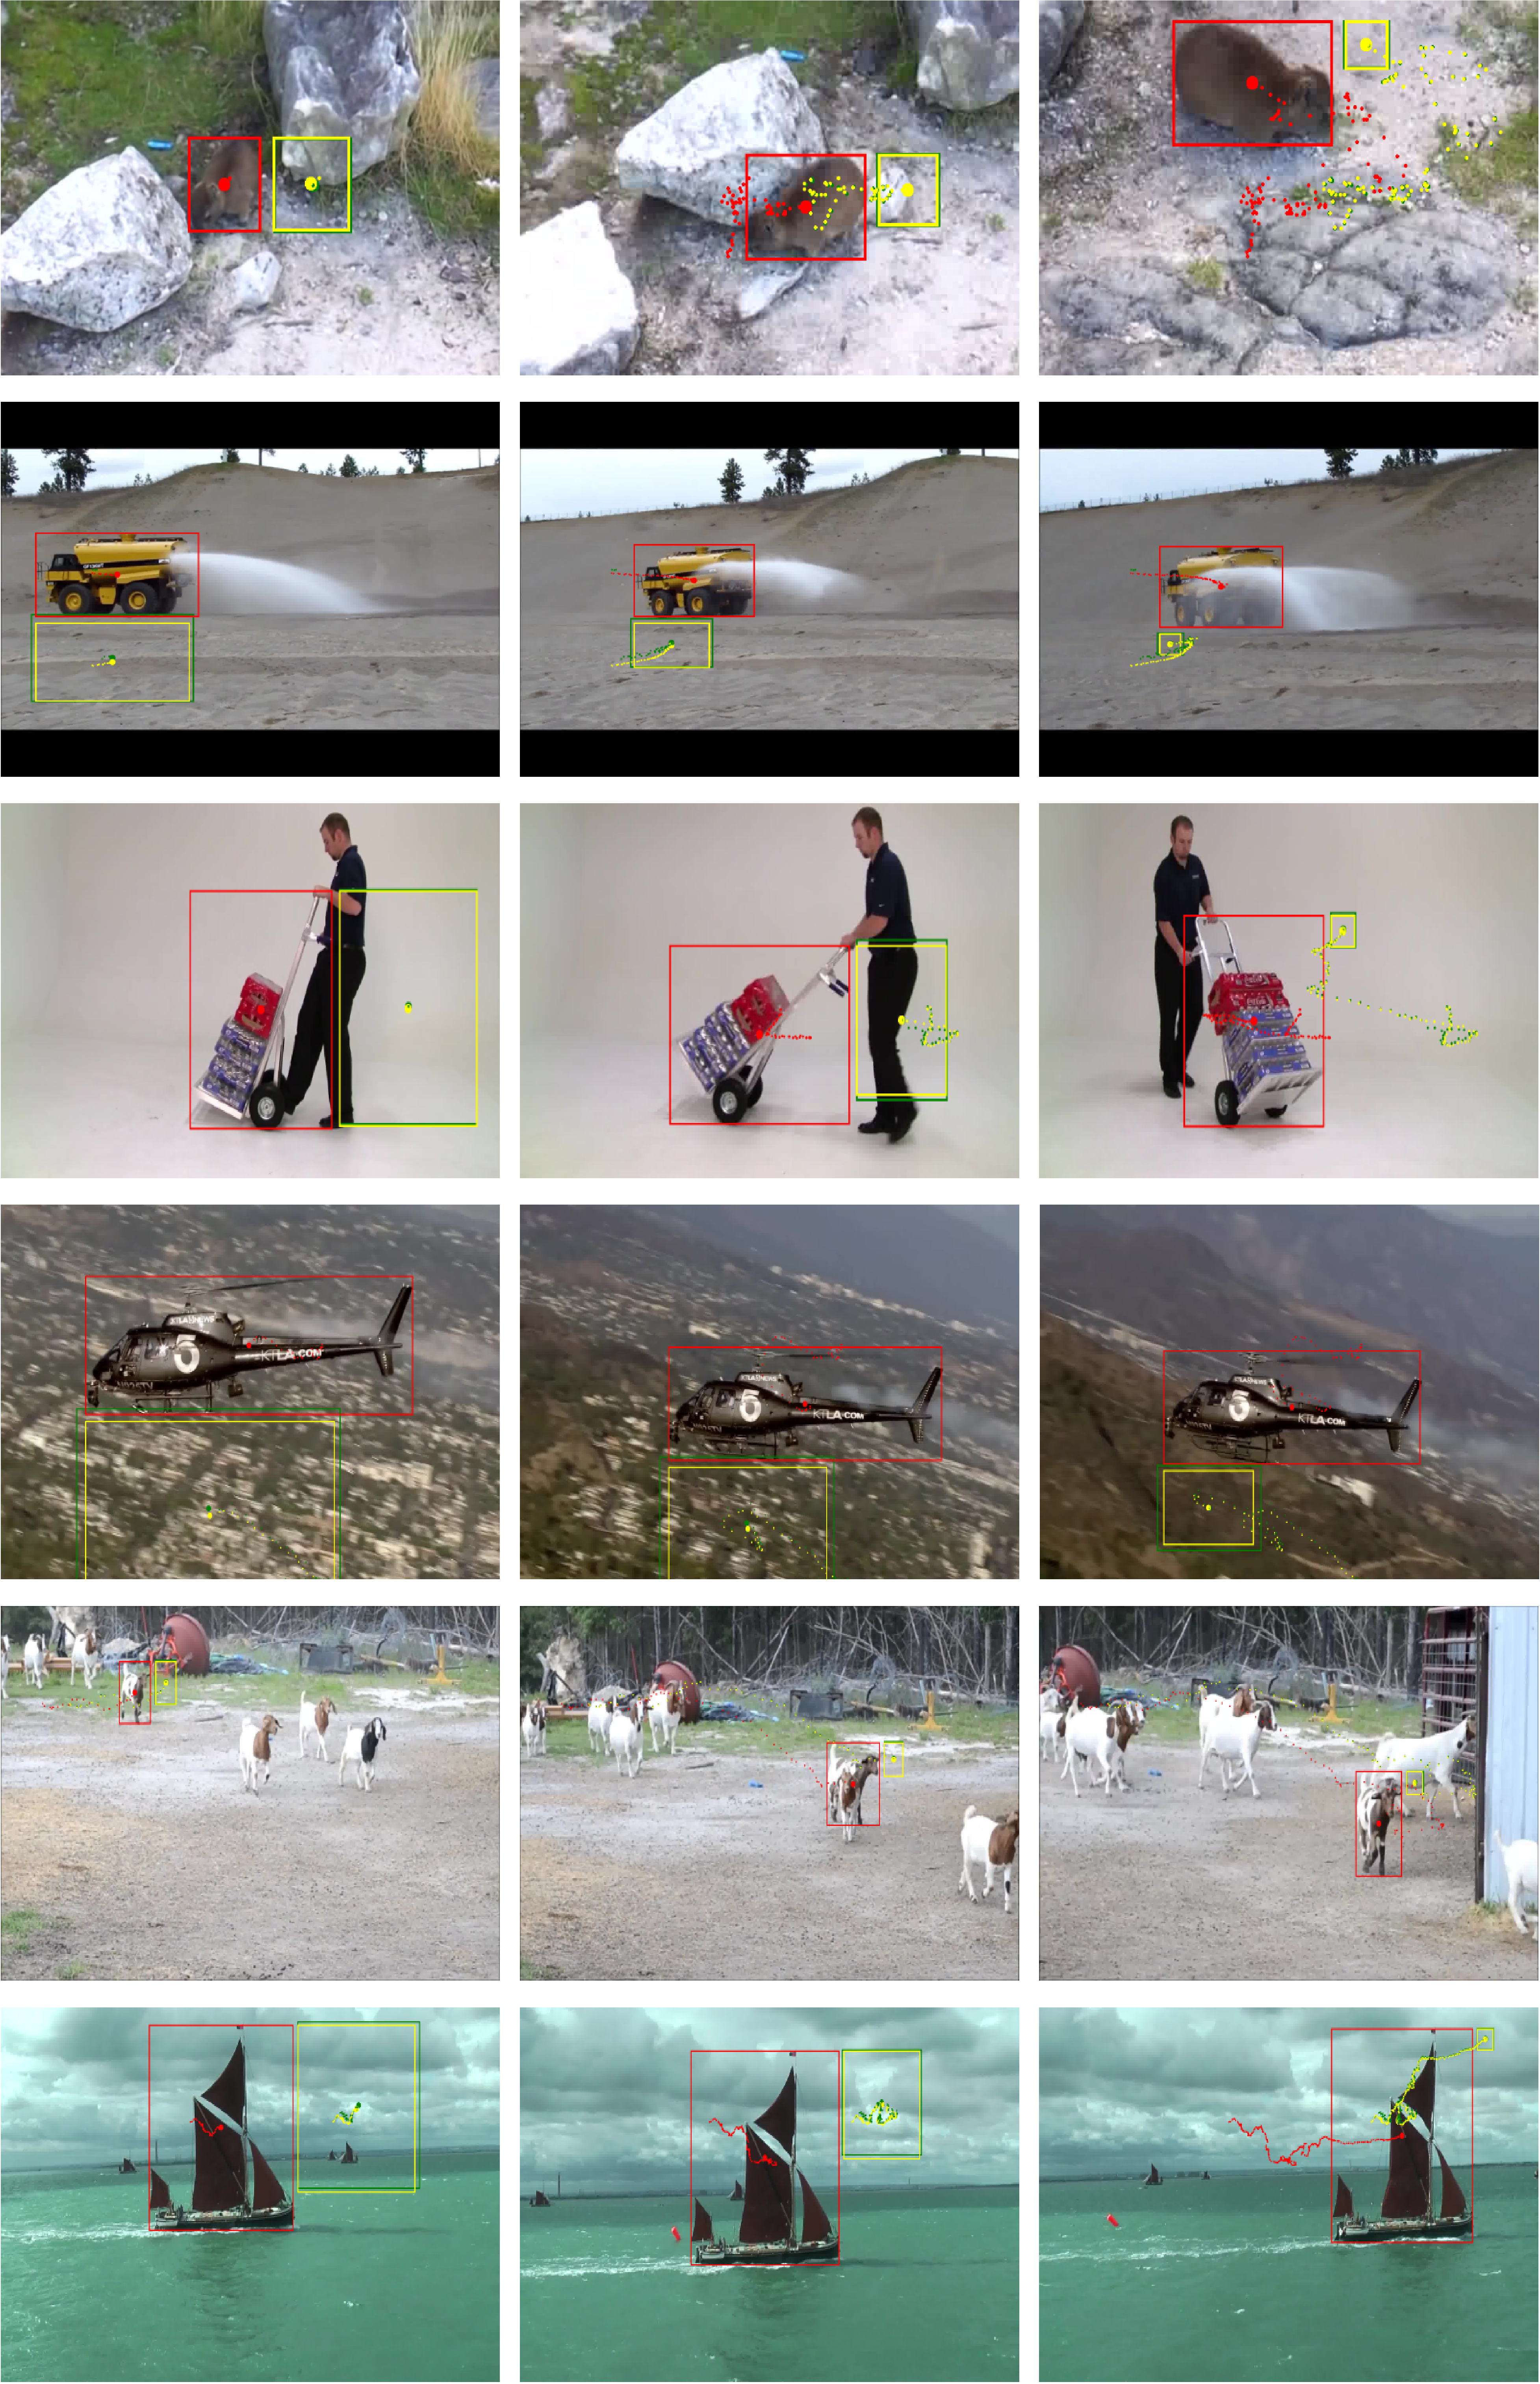
\includegraphics[width=1.0\textwidth]{Img/attack/txt_visualize.pdf}
\caption{基于 GOT-10k \cite{GOT-10k} 验证集的对抗攻击效果展示。红色边框表示真实目标位置,黄色边框表示预定义的虚假目标位置,绿色边框表示跟踪器在对抗视频上预测的目标位置。}
\end{figure}

\textbf{总体攻击结果} 我们在目标跟踪数据集上测试了针对性攻击方法的性能,并将总体结果收集在表 \ref{tab:attack_benchmark results} 中。结果表明,基线跟踪器 SiamFC++ 可以在所有视觉目标跟踪数据集上达到最先进的性能,并且可以实时运行(在 GTX 1080Ti GPU 上约为 58 FPS)。但是,这种实时性能的代价是计算量大,导致跟踪系统会占用大部分计算资源,因此有必要开发一种几乎不增加计算成本的攻击方法来欺骗跟踪系统而不会争用计算资源。如表 \ref{tab:attack_benchmark results} 所示,我们的攻击方法可以满足该要求,并通过误导跟踪器遵循预定义的虚假轨迹来有效地欺骗 SiamFC++ 跟踪器。此外,相对于虚假轨迹而言,较高的 AO 和 Precision 得分表明对抗性信息在不引起任何怀疑的情况下执行有效攻击(图 \ref{fig:attack_vis})。

\begin{table}[t]
\centering
\caption{在数据集 GOT-Val 上验证对抗性信息在不同主干网络之间的可迁移性。}
\begin{tabular}{c cc cc cc} 
\toprule
\multirow{3}{*}[-6pt]{主干网络} & \multicolumn{2}{c}{原始视频}    & \multicolumn{4}{c}{扰动视频}                                        \\ 
\cmidrule(lr){2-3} \cmidrule(lr){4-7}
                          & \multicolumn{2}{c}{真实轨迹} & \multicolumn{2}{c}{真实轨迹} & \multicolumn{2}{c}{虚假轨迹}  \\ 
\cmidrule(lr){2-3} \cmidrule(lr){4-7}
                          & AO    & SR                           & AO    & SR                           & AO    & SR                           \\ 
\midrule
GoogLeNet \cite{GoogLeNet}& 0.760 & 0.897                        & 0.035 & 0.023                        & 0.818 & 0.890                        \\
AlexNet \cite{AlexNet}    & 0.720 & 0.850                        & 0.196 & 0.227                        & 0.572 & 0.640                        \\
ShuffleNet\cite{ShuffleNet}& 0.766 & 0.888                        & 0.554 & 0.656                        & 0.135 & 0.134                        \\
\bottomrule
\end{tabular}
%}
\label{tab:backbone}
\end{table}

\textbf{训练损失对攻击性能的影响} 我们实施了一系列实验来分析和评估每个损失成分的贡献。
在表 \ref{tab:attack_loss} 中,我们报告了在 GOT-Val 数据集上的攻击结果。该结果反映了使用公式 \ref{eq:loss} 中损失项的不同组合训练得到的不同扰动的攻击性能差异。
当仅利用质量评估损失生成对抗性信息时,跟踪器相对于真实轨迹的 AO 值从 0.760 下降至 0.703,说明质量评估损失可使跟踪器的性能发生轻微下降。这是因为利用质量评估损失生成的扰动信息干扰了跟踪器选择最佳目标框的能力。
然而,跟踪器相对于虚假轨迹的 AO 值仅为 0.044,说明仅使用质量评估损失生成的扰动几乎无法令跟踪器沿指定轨迹生成跟踪框。
当仅利用回归损失生成对抗性信息时,跟踪器相对于真实轨迹的 AO 值从 0.760 下降至 0.165,说明回归损失可使跟踪器的性能发生较大下降。这是因为利用回归损失生成的扰动信息破坏了跟踪器对真实目标边框位置的预测能力。
当仅利用分类损失生成对抗性信息时,跟踪器相对于真实轨迹的 AO 值从 0.760 下降至 0.086,相对于虚假轨迹的 AO 值高达 0.718。这是因为使用分类损失生成的扰动信息使跟踪器定位到虚假目标,而非真实目标的位置。
总而言之,所有损失项都是有益的,而分类项比质量评估项更重要。

\begin{table}[t]
\caption{在视觉目标跟踪数据库 OTB2015 上验证对抗性信息在不同跟踪架构之间的可迁移性。}
\centering
\begin{tabular}{ccccc} 
\toprule
\multirow{2}{*}[-2pt]{跟踪器} & \multicolumn{2}{c}{原始视频} & \multicolumn{2}{c}{对抗视频}  \\
\cmidrule(lr){2-3} \cmidrule(lr){4-5}
                          & AO & Precision              & AO & Precision                   \\
\midrule
SiamRPN++ \cite{SiamRPN++}& 0.676   & 0.879                  & 0.518   & 0.691                       \\
SiamRPN \cite{SiamRPN}    & 0.666   & 0.876                  & 0.379   & 0.506                       \\
\bottomrule
\end{tabular}
%}
\label{tab:arch}
\end{table}

\textbf{训练迭代次数对攻击性能的影响} 表 \ref{tab:attack_iter} 展示了算法的训练迭代次数对攻击效果的影响。可以观察发现随着迭代次数的增加,相对于虚假轨迹的 AO 值明显升高,而相对于真实轨迹的 AO 值明显下降。这说明了本章提出的端到端训练流程的有效性。
经过大约 30000 次训练迭代后,所产生的扰动会使跟踪器无法跟踪 GOT-Val 中的大多数目标,相对于真实轨迹的 AO 从 0.760 下降到 0.035。
我们注意到,在训练周期开始时(训练迭代次数小于 2048),AO 的下降速度明显快于后期。这证明了我们的端到端训练方案的快速收敛能力。

为了验证为模板图像生成的扰动是否难以感知,我们对扰动后的模板图像质量进行了评估分析。扰动后的模板图像质量由指标 SSIM 进行评估。如表 \ref{tab:attack_iter} 所示,随着训练的进行,扰动后模板图像的 SSIM 值逐渐下降,这说明由于学习的对抗性扰动被添加至干净的模板图像上,导致扰动后的模板图像差异与原始模板图像的差异逐渐增大。随着训练的继续进行,当 SSIM 降至 0.88 后便不再继续下降,这说明网络的训练已经收敛,扰动后的模板图像差异与原始模板图像的差异不再继续增大。SSIM 的取值范围为 0 到 1,如果 SSIM 越接近 1,说明扰动后的模板图像差异与原始模板图像的差异越小,即为模板图像生成的扰动越难以感知;如果 SSIM 越接近 0,说明扰动后的模板图像差异与原始模板图像的差异越大,即为模板图像生成的扰动越容易感知。本算法收敛后的 SSIM 值为 0.88,说明扰动后的模板图像差异与原始模板图像的差异较小,即为模板图像生成的扰动较难感知(参见图 \ref{fig:1})。

\begin{table}[t]
\centering
\caption{通过在评测库 OTB2015 上的跟踪精确度对比本章提出的攻击算法与相关攻击算法的有效性。}
\setlength{\tabcolsep}{3pt}
\begin{tabular}{@{}ccccccc@{}}
\toprule
\multirow{2}{*}[-2pt]{攻击方法} & \multirow{2}{*}[-2pt]{跟踪器} & \multirow{2}{*}[-2pt]{攻击时间 (ms)} & \multirow{1}{*}[-2pt]{原始视频} && \multicolumn{2}{c}{对抗视频} \\
\cmidrule{4-4} \cmidrule{6-7}
 &  &  & 真实轨迹 & & 真实轨迹 & 虚假轨迹 \\ \midrule
CSA  \cite{CSA} & SiamRPN \cite{SiamRPN} & 4720 & 0.851 & & 0.458 & - \\
FAN \cite{FAN} & SiamFC \cite{SiamFC} & 10 & 0.720    & & 0.180&0.420 \\
TTP \cite{TTP} & SiamRPN++ \cite{SiamRPN++} & 8 & 0.910  && 0.080&0.692 \\
\midrule
本章算法 & SiamFC++ \cite{SiamFC++} & 0 & 0.861  & & 0.048&0.928 \\ \bottomrule
\end{tabular}%
\label{tab:untargeted}
\end{table}

\subsection{对抗性信息的可迁移性分析}

\textbf{不同主干网络的迁移能力} 为了验证对抗性信息在不同主干网络上的迁移能力,我们将扰动应用于 SiamFC++ 的另外两个不同的主干,即 ShuffleNet \cite{ShuffleNet} 和 AlexNet \cite{AlexNet}。
实验结果显示在表 \ref{tab:backbone} 中。对于 SiamFC++\_AlexNet,相对于真实轨迹的 AO 从 0.72 下降到 0.196。然而,我们的扰动不能很好地推广到 SiamFC++\_ShuffleNet,我们推测这是由于 ShuffleNet 中特殊的组卷积和通道混洗操作所致。

\textbf{不同跟踪架构的迁移能力} 为了验证对抗性信息在不同跟踪架构上的迁移能力,我们将扰动应用于另外两个基于锚框的最新跟踪器:基于 AlexNet 的 SiamRPN \cite{SiamRPN} 和基于 ResNet 的 SiamRPN++ \cite{SiamRPN++}。
SiamRPN 使用 RPN 网络在响应图上执行位置回归和目标分类。 SiamRPN++ 在使用 ResNet 主干进行有效训练的基础上,执行逐层和深度聚合,以提高准确性。实验结果显示在表 \ref{tab:arch} 中。在 SiamRPN 中,相对于真实轨迹的 AO 从 0.666 降低到 0.379,而 SiamRPN++ 的性能从 0.676 降低到 0.518。结果表明,即使将生成的扰动应用于基于锚框的跟踪器,我们的对抗性信息也具有很好的可迁移性。

\subsection{与当前主流对抗攻击方法的比较}

我们将本章提出的孪生网络攻击方法与最新的攻击方法进行了比较,包括基于 AlexNet 的非针对性攻击方法 CSA \cite{CSA},和其他两种针对性攻击方法:基于 AlexNet 的 FAN \cite{FAN} 和基于 ResNet50 的 TTP \cite{TTP}。
我们在表 \ref{tab:untargeted} 中报告相对于真实/虚假轨迹的精确度得分。
CSA \cite{CSA} 是一种称为冷却收缩攻击(cooling-shrinking attack)的孪生跟踪攻击方法。CSA 可以抑制反映目标位置的热图上的峰值区域,用于攻击跟踪器的目标定位能力;CSA 还可同时迫使跟踪器预测的边界框缩小,用于攻击跟踪器的边框回归能力。然而,该方法需要为每一帧运行生成网络以得到对抗性信息,因此攻击时间高达 4720 毫秒,难以满足实时跟踪的需求。CSA 可使相对于真实轨迹的精确度得分从 0.851 下降至 0.458,攻击性能较为有限。由于算法设计的局限性,CSA 无法执行目标跟踪的针对性攻击。
在文献 \cite{FAN} 中,Liang 等人提出了一种快速攻击网络(fast attack network,FAN),用于攻击 SiamFC 跟踪器。为了执行非针对性攻击,FAN 提出了漂移损失,使得跟踪器对目标位置的预测发生偏移。随着时间的推移,跟踪误差不断累积,直到跟踪器完全丢失目标。为了执行针对性攻击,FAN 提出了嵌入特征损失,用于提高对抗样本特征与特定轨迹区域特征的相似性。FAN 可使相对于真实轨迹的精确度得分从 0.720 下降至 0.180,具有较好的非针对性攻击性能。然而,该方法相对于虚假轨迹的精确度得分仅为 0.420,针对性攻击性能较为有限。与 CSA 类似,FAN 同样需要为每一帧运行生成网络以得到对抗性信息。
在文献 \cite{TTP} 中,Nakka 等人提出了一种可时序迁移扰动(temporally transferable perturbations,TTP),用于攻击 SiamRPN++ 跟踪器。TTP 仅从模板图像生成单个对抗性扰动,并将该扰动添加到视频的每个搜索图像中,以执行针对性攻击。TTP 可使相对于真实轨迹的精确度得分从 0.910 下降至 0.080,具有较好的非针对性攻击性能。然而,该方法相对于虚假轨迹的精确度得分仅为 0.692,针对性攻击性能较为有限。此外,该方法需要为每段视频运行生成网络以得到对抗性信息,因此需要占用目标跟踪平台的计算资源和存储资源,难以部署至资源受限的嵌入式平台中。
我们的方法可使相对于真实轨迹的精确度得分从 0.861 下降至 0.048,相对于虚假轨迹的精确度得分高达 0.928,性能上明显优于其他方法,且仅需要执行加法操作和图像粘贴操作,无需梯度优化或网络推断,即可为任意视频生成对抗性信息。

\section{本章小结}

在本章中,我们提出了一种针对孪生跟踪器的视频无关的针对性攻击方法,旨在通过向模板图像添加不可感知的扰动并将虚假目标(即小的对抗补丁)根据预定轨迹粘贴到搜索图像中来攻击跟踪器,以便跟踪器输出虚假目标而非真实目标的位置。
通过损失函数的巧妙设计,我们的对抗性信息不仅可以误导跟踪器的分类结果,还可以误导跟踪器的回归结果。
%所提出的对抗性信息具有通用性,因此可以用于扰动任意视频,而无需进行额外计算。
所提出的对抗性扰动信息通过离线的大规模视觉目标跟踪数据集训练得到,可在占用极少计算资源的情况下对任意视频进行有效攻击。
我们在目前比较流行的视频跟踪标准评测库上对所提出的对抗性信息的有效性进行了评估,实验证明所提出的视频无关的对抗性信息能够有效执行攻击,同时在不同主干网络和不同跟踪框架之间具有良好的可迁移性。